\chapter{Relativistic results}\label{ch:rel}

Chapter~\ref{ch:nonrel} ended with a number that undermines its own premise: a coherent speed of $0.47c$ to $0.87c$ at the ends of the certified windows. The next step was therefore to give the continuum solvers a relativistic electron and to run the HHS resonance again. The same step needed an independent relativistic particle code, because the question we want to answer, how large the electron heating of HHS is and what produces it, can only be asked of a code that has the noise HHS have. The chapter reports four calculations that share the set-up of Chapter~\ref{ch:hhs}: an exact homogeneous relativistic driven oscillator; a relativistic grid Vlasov solver; a relativistic version of the Hermite solver; and a relativistic PIC. It then states what they agree on, which is the collapse of the mean-field response, and what they do not, which is the heating, by a factor that is at its smallest a factor of two and at its largest of order $10^{2}$.

\section{The exact relativistic driven oscillator}\label{sec:c10-homog}

The role of relativity can be seen in a model small enough to be solved on the page. A spatially uniform plasma under a uniform drive responds only through its $k=0$ moments, and for cold electrons with $q/m=-1$ in units $c=\wpe=1$ the momentum per unit mass $u=\gamma v$ obeys $\dot u=-(\bar E+E_0\cos\omega t)$ while the field obeys $\dot{\bar E}=-\bar J=nv$ up to the ion term. The exact relativistic kinetic version replaces $v$ by the average of $u/\gamma(u)$ over the distribution, which depends on the whole distribution, not on a single mean; it is a closed set of ordinary differential equations for the distribution of $u$ because a uniform field only translates it, and the exact solution is recorded to $\wpe t=5000$ (\texttt{studies/relgrid/homog.json}).

The derivation of the effect is in Section~\ref{sec:relativistic}, where a cold oscillator is shown to lose a fraction $\tfrac3{16}p_0^2$ of its frequency at momentum amplitude $p_0$ (Eq.~\eqref{eq:duffing}), a hot plasma to lose $\tfrac34\theta$ at temperature $\theta=v_{te}^2/c^2$, and the slow-flow model built from both to reproduce the exact homogeneous kinetic integration. We take that integration, which is made for the note by \texttt{note/make\_note\_figures.py} and recorded in \texttt{note/figures/k0\_relativistic.json}, as the reference value: the $10\,\%$ departure of $\Wext$ from the nonrelativistic law falls at $\wpe t=392.3$ for $\vq=0.03$ and at $1428.8$ for $10^{-3}$. The script \texttt{note/check\_relosc.py} confirms the $3/16$ coefficient by direct integration of the cold oscillator, with $(1-\omega)/v_m^2=0.1877$ to $0.1956$ for $v_m=0.05$ to $0.29$.

The cold estimate is nonetheless worth keeping as an illustration of what the thermal shift does. Under resonant driving the quiver speed grows as $v_m\simeq v_q t/2$ with $v_q=\vq\,v_{te}$ the drive in units of $c$, so the cold shift accumulates the phase $\varphi(t)=\int_0^t\tfrac3{16}(v_qt'/2)^2\,\mathrm dt'=v_q^2t^3/64$, which reaches one radian at $\wpe t=(64/v_q^2)^{1/3}$. For $\vq=0.03$ this is $414$, within $6\,\%$ of the exact $392$ and with the right scaling $v_q^{-2/3}$. For $\vq=10^{-3}$ it is $4000$, three times the exact $1429$. The failure is the content of the thermal term: the quiver speed at $\wpe t\simeq1400$ is only $0.02c$, and a Maxwellian of temperature $10^{-3}mc^2$ has by itself a frequency shift of $7.5\times10^{-4}\wpe$ that accumulates a radian in about $1.3\times10^3\wpe^{-1}$ whatever the drive. In the slow-flow model of Chapter~\ref{ch:plasma} the cold version gives $437$ for the strong drive and no collapse for the weak one, while the version with the thermal term gives $397$ and $1438$, so the thermal shift is tested and not assumed. In the nonrelativistic grid with the same weak drive the work does not depart from the linear law at all up to $\wpe t=3000$, while the mean-field energy is $0.71$ of its linear value there (against $0.50$ for the relativistic grid).

The relativistic effect is also large. In the exact homogeneous problem the relativistic $\Wext$ is $0.0056$ of the nonrelativistic one at $\wpe t=1000$ for $\vq=0.03$, and a check in a relativistic code discriminates strongly: the nonrelativistic law misses $\Wext$ by $38\,\%$ at $\wpe t=500$ (record \texttt{studies/relhhs/gates\_g1.json}). The relativistic mass increase of the coherently quivering electrons detunes the uniform resonance by itself, in a calculation with no fluctuations, no instability and no density modulation. That is a different mechanism from the one HHS describe, and the rest of the chapter asks what it leaves unexplained.

\section{The relativistic grid}\label{sec:c10-grid}


The relativistic grid solver (\texttt{studies/relgrid.py}) integrates the one-dimensional, one-momentum-dimension Vlasov--Amp\`ere system for electrons and ions on a fixed $(x,u)$ grid, with $u=p/mc$ as the momentum variable, so that the force term is unchanged and only the streaming velocity $u/\gamma$, the current and the kinetic energy $(\gamma-1)mc^2$ change. Space is spectral with $N_x$ Fourier modes and the two-thirds mask, momentum uses 4096 nodes, and the step is $0.02\,\wpe^{-1}$ with an iterative or Taylor midpoint. It has no Hermite truncation and no closure, a property that matters: it can lose positivity, but it cannot develop the truncation instability of Chapter~\ref{ch:nonrel}. Seeds are either deterministic, like those of the Hermite code, or built from shot noise of a stated particle number per cell.

The gates were declared in \texttt{studies/relgrid\_gates.py} before any run. The nonrelativistic limit reproduces the earlier nonrelativistic record to $1.5\times10^{-10}$ (gate $\le10^{-9}$) and the laboratory and oscillation frames agree to $1.5\times10^{-10}$. The homogeneous problem agrees with the exact kinetic ODE with a second-order error (the $\Delta t^2$ ratio is $3.99$) and Richardson-extrapolated errors of $5.6\times10^{-7}$ in $\bar E$, $5.2\times10^{-7}$ in $U_e$, $3.4\times10^{-7}$ in $W$ and $7\times10^{-8}$ rad in phase. Three declared checks failed. The Landau-root check C fitted the real part of $E_1$, which for a real density seed is noise, and failed; the replacement C2, declared before it was run and using the imaginary part, passes with errors of $8.9\times10^{-5}$ in frequency and $4.5\times10^{-4}$ in damping at $k\lambda_{De}=0.3,0.4$, closer to the relativistic roots ($1.15849-0.01203i$ at $k\lambda_{De}=0.3$) than to the nonrelativistic ones ($1.16001-0.01260i$). The ledger gate D, a defect of at most $10^{-4}$ of the work, failed: $2.3\times10^{-4}$ for the deterministic run at $\Delta t=0.02$, with 15 of 16 runs above $10^{-4}$. Its companion D2, that the defect should fall by a factor of $3$--$5$ when $\Delta t$ is halved, also failed with a ratio of $8.0$ (the value at $\Delta t=0.01$, $2.9\times10^{-5}$, does pass). The grid ledger is therefore weaker than that of the Hermite code by about four orders of magnitude, and this is carried into every grid result below. Refinement pairs in $N_x$, momentum nodes and time step agree to $\wpe t=1000$ under the $10\,\%$ rule.


The collapse times of the grid follow the homogeneous prediction. For the deterministic seed at $\vq=0.03$, $N_x=32$, the work leaves the linear law by $10\,\%$ at $\wpe t=392$. The mean-field energy relative to its linear value is $0.854$ at $\wpe t=500$ and $0.041$ at $1000$, which corresponds to $3.7\,\Eth$ (that is $1.9\times10^{-3}n_em_ec^2$) of absolute mean-field energy at $1000$. HHS show, by our reading of the logarithmic plot, a mean-field energy of about $10^{-3}$ near $\wpe t\simeq800$ and below $10^{-4}$ at $1000$ in the same units; the timing of the relativistic collapse is consistent with theirs, the late level of the deterministic grid is about a factor $20$ above theirs. With shot-noise-like seeds the collapse time is $367$--$392.5$, depending on the particle number of the seed and on $N_x$, among the seeds that stay valid long enough to define it; the nonrelativistic grids with the same noise collapse at $769.5$--$866.5$. The deterministic nonrelativistic Hermite code shows no collapse in its windows. At $\vq=10^{-3}$ the relativistic grid departs at $1309.5$ (deterministic) and $1413.5$ (shot noise), and its mean-field energy is $0.50$ of the linear value at $\wpe t=3000$, with a heating of $0.09\,\Eth$ (nonrelativistic: $0.71$ and below $0.3\,\Eth$). Relativity is thus both necessary and sufficient for a collapse before $\wpe t\simeq800$ in the continuum models: necessary because the nonrelativistic ones do not collapse before $770$ even with noise, and sufficient because the deterministic relativistic grid collapses at $392$ with no instability at all. This is the first of the two results to which the rest of the note returns.


The HHS heating of $50\,\Eth$ is the second result to be reproduced, and the deterministic grid does not do it: the electron energy gain in the HHS measure is $0.018\,\Eth$ at $\wpe t=500$ and $0.056\,\Eth$ at $1000$, with the minimum of $f$ equal to $-3\times10^{-12}$, so that nothing is wrong numerically. Detuning switches off the mean field, and it does not heat. The remaining candidate is a fluctuation level. The grid was therefore run with density seeds drawn from the shot noise of $N_{\rm pc}$ particles per cell. For $N_{\rm pc}=205$, the PIC particle number, the run is invalid: $f<-10^{-3}$ already within $\wpe^{-1}$ of the start, the noise amplitude of the lowest modes being comparable to the thermal energy; it is kept and labelled so. For $N_{\rm pc}=2.05\times10^{5}$ (a seed of $U_{k0}=7\times10^{-7}$) the heating begins at about $\wpe t=600$ and the values at $1000$ are $15\,\Eth$ ($N_x=32$), $51$ ($N_x=64$) and $30$ ($N_x=128$), with $50$ for $N_{\rm pc}=2.05\times10^{4}$ at $N_x=32$ and $209$ for the nonrelativistic control. These numbers are of the HHS size and suggestively so, and they are not results. In all of these runs $f<-10^{-3}$ appears between $\wpe t=240.5$ and $407.5$, the box edge fraction exceeds $10^{-6}$ between $350$ and $500$, and the ledger exceeds $10^{-4}$ between $350$ and $510$. The heating at $\wpe t=500$ is $5$--$10\,\Eth$ for $N_x=64,128$ and the valid window ($t<350$) has less than $0.01\,\Eth$. The question whether the cascade at the high $k$ resolved by $N_x=64$ and $128$ would heat if the code could survive remained open. The answer from the grid is therefore: the heating of HHS is not reproduced within validity, and cannot be assessed beyond it.

A finer Fourier range was tried in the nonrelativistic grid (the \texttt{hkr} study), reaching $N_x=1024$ and $k\lambda_{De}=1.69$, since HHS' modulational and decay instabilities populate modes up to the inverse Debye length. The deterministic gain at $\wpe t=1000$ is $2.3\,\Eth$ for $N_x\ge512$ (the chains at $N_x=256,640,1024$ agree over their certified windows), about 20 times smaller than the HHS value. With shot noise the grid loses positivity at $\wpe t=69$--$163.5$ and has gained $0.013\,\Eth$ by then, whatever $N_x$, so the Fourier range alone does not explain the heating (declared question Q1 of the study). Five of the validation checks of the study at $k\lambda_{De}=1$ failed as specified and are recorded in \texttt{studies/hkr/validation*.json} together with the follow-ups that were declared after each.

\section{The relativistic Hermite model}\label{sec:c10-herm}


The Hermite model was extended in two steps. In the variable $u=p/mc$ the force term is unchanged and only the streaming, the current and the kinetic energy involve $v(u)=u/\gamma$. The velocity operator $V=P\,{\rm diag}(v(u_0+a\lambda_j))P^T$ is diagonalized once in the Hermite basis, with the same eigendecomposition as the exact Lawson streaming factor of the nonrelativistic code, so that streaming and the current remain matrix functions of one decomposition. A relativistic option was then added to the parent solver (SPECTRAX PR 88) and the pump frame was extended to it, at the pin \texttt{6a6606b} of \texttt{integration/dark-baseline-2}. The field-scaled closure is a diagonal damping outside the kernel and is unchanged, and it remains exact in the Lawson factor. Three things are not supported and are refused by the code: the exact streaming factor in the relativistic case (streaming is explicit), Dougherty collisions, and the magnetic term in more than one transverse axis (the three-velocity case couples axes through $\gamma$ and would cost $O(N^4)$). Nonrelativistic runs are bitwise unchanged.

The gates were again declared first. In a limit with $c\to\infty$ the right-hand side agrees with the nonrelativistic solver to $10^{-15}$; a single gyrating electron matches the exact relativistic frequency to $2\times10^{-10}$; the magnetic force does no work to $3\times10^{-15}$; and the ledger including $(\gamma-1)mc^2$ closes to $6.6\times10^{-10}$ for an electron driven to $0.13c$ and to $8\times10^{-9}$ at $0.83c$. The spectrum check c failed as declared, because the discrete spectrum of a truncated Hermite matrix is undamped and the control failed in the same way (the declaration was wrong); the replacement c2 on the response function passes at $3\times10^{-5}$. The nonlinear $1\mathrm{D}2\mathrm{V}$ run with a transverse field failed at $\wpe t\simeq8$ with a NaN from the truncation instability, which is not a relativistic effect (the frozen-field growth is $4.7$ relativistic against $4.9$ nonrelativistic); the variant with a hypercollision of strength 10, declared afterwards, closes at $6.8\times10^{-6}$ and removes $0.7\,\%$ of the energy change at a mean speed of $0.59c$.

The production study then ran the HHS resonance in eight configurations, $N_x\in\{32,64\}\times N_n\in\{64,128\}\times c\in\{16,64\}$, to $\wpe t=1000$. The declared gates all pass. G1, the homogeneous limit against the exact kinetic ODE for $\wpe t\le500$ at $N_n=64,128$: $1.7\times10^{-9}$ and $2.5\times10^{-9}$ in $\bar E$, $5.5\times10^{-10}$ and $7.8\times10^{-10}$ in $\Wext$, $1.6\times10^{-9}$ and $2.3\times10^{-9}$ rad in phase, against a threshold of $10^{-6}$; the nonrelativistic ODE misses $\Wext$ by $38\,\%$ as noted. G2, that 12 refinement pairs agree to $10\,\%$ in $\Delta K_e$ and $\Wext$ to a declared $400$, passes to $1000$. G3, positivity, and G4, the ledger including the rest-mass term to $10^{-4}$, pass with a maximum of $1.8\times10^{-8}$ for $t\le400$. The fraction of the energy in the top third of the Hermite ladder is below $3\times10^{-8}$.


The work leaves the linear law by $10\,\%$ at $\wpe t=392.5$ in all eight runs, to the resolution of the sampling, against $392$ for the grid. The mean-field energy relative to the linear law is $0.855$ at $500$ (grid $0.854$) and $0.0409$ at $1000$ (grid $0.0407$). The HHS measure of the thermal gain is $0.0177\,\Eth$ at $500$ and $0.056\,\Eth$ at $1000$, identical in all eight runs to three digits and identical to the deterministic grid ($0.0559$). Two independent discretizations, one with a closure and one without, agree on the mean field and on the heating to the digits shown. This is the strongest evidence in the note that the continuum answer to the deterministic problem is right, and it is also the evidence that the deterministic problem does not heat.

Two follow-ups were declared after the production gates and both failed. F1, certification to $\wpe t=2000$, fails: $f_e<-10^{-3}$ appears at $1528$ and $1584.5$ for the two base runs, the ledger exceeds $10^{-4}$ at $1855$ for $N_x=32$, and the $N_x=64$ run was stopped at $1800$ once the horizon had been fixed; the pairs do not disagree. The heating stays below $0.7\,\Eth$ throughout. The model is therefore certified to about $\wpe t=1530$--$1585$, past the validity of the shot grid ($t<350$) and short of the declared $2000$. F2, shot-noise seeds with the recipe of the grid, fails: with $N_{\rm pc}=103$, the PIC value, $N_x=32$, $N_n=64$ has $f_e<-10^{-3}$ at $\wpe t=0.5$, the ledger above $10^{-4}$ at $10.5$ and a positivity stop at $143$, and the $N_x=64$, $N_n=128$ run never finished its first 100-unit chunk and was killed after 70 minutes; with $N_{\rm pc}=2.05\times10^{5}$ positivity fails at $367$ ($N_x=32$) and $265$ ($N_x=64$), with stops at $660$ and $380$, against $246$--$278$ for the grid. The Hermite model reproduces the deterministic relativistic collapse to three or four digits and a ledger of $10^{-8}$, and cannot reach the PIC regime before losing positivity. The cost of a $T=1000$ run is $2$--$19$ minutes on one thread under load.

\section{The relativistic PIC}\label{sec:c10-pic}


The comparison that matters for the heating needs a particle code. The independent test is one. Dark-JAX-in-Cell (commit \texttt{d547579}) on JAX-in-Cell (\texttt{2d693cb}) has a relativistic Boris pusher of the Vay family. The configuration reproduces what HHS state about their own: 1000 cells of $0.04\,c/\wpe$ in a box $L=40\,c/\wpe$, $m_i/m_e=1836$, $T_e=T_i=10^{-3}m_ec^2$, a uniform prescribed drive with $\vq=0.03$ at the cold frequency, quadratic shape functions and $\Delta t=0.02\,\wpe^{-1}$; the same code with the Newtonian momentum is the control. Before any production run the pusher was tested on single particles (S1--S3: pure electric and pure magnetic motion exact, the $\mathbf E\times\mathbf B$ drift error $1.7\times10^{-4}$ and second order), and in a pilot to $\wpe t=100$ the Gauss-law and continuity residuals were at $10^{-14}$. The first twelve production runs (three seeds each, to $\wpe t=2000$) passed G1, G2, G3, G6, G7 (quintic shape) and G9 (no-drive control), and failed G4 (the heating at 412 particles per cell was $19\,\%$ above that at 103), G5 (a cell of $0.02$ raised it by $19\,\%$ and $18\,\%$ at 400 and 600) and G10 (the $N_x=32$ Hermite record lies one to two orders of magnitude below the PIC). These failures prompted the convergence ladder rather than a conclusion.


The ladder was declared in \texttt{studies/relpic/conv\_gates.py} (follow-up in \texttt{conv\_followup\_gates.py}) and run on CPU with 15 new runs. Its results for the HHS measure at $\wpe t=1000$ in units of $\Eth$ are given in Table~\ref{tab:c10-pic}. In particles per cell at $\Delta x=0.04$ the heating is $21.5\pm0.6$ (103), $23.7$ (206), $24.6\pm2.0$ (412, five seeds), $25.0$ (824) and $24.9$ (1648): a rise of about $15\,\%$ between 103 and 412 and then a plateau with successive changes of $1.4\,\%$ and $0.1\,\%$. Halving the cell at 103 particles per cell gives $24.1$ ($0.02$) and $24.3$ ($0.01$), a change of $0.8\,\%$ between the two. Quintic shape functions at 412 give $25.7$, and halving the time step at 103 gives $21.1$ against $21.5$. The gates C1 to C4 (successive differences within $5\,\%$ or twice the seed spread) pass; their tolerances contain an allowance of $2\sqrt2$ times the seed standard deviation, which at 412 particles per cell is $2.0\,\Eth$. At $\wpe t=2000$ and 412 particles per cell the heating is $28.0\pm3.7$. The plateau is $\simeq25\,\Eth$, half of the re-digitized HHS value of $50.1$ ($52.7$ at $2000$).

\begin{table}[t]
\centering
\caption{PIC electron heating in the HHS measure, $\Delta E_e/\Eth$ at $\wpe t=1000$ (trailing $200\,\wpe^{-1}$ mean), $\vq=0.03$, relativistic unless stated, quadratic shape, $\Delta x=0.04$, $\Delta t=0.02$ except where varied (record \texttt{studies/relpic/conv\_summary.json}). The $\pm$ is the standard deviation over seeds.}\label{tab:c10-pic}
\small
\begin{tabular}{@{}lc@{}}\toprule
variation & $\wpe t=1000$\\\midrule
103 ppc (3 seeds) & $21.5\pm0.6$\\
206 ppc & 23.7\\
412 ppc (5 seeds) & $24.6\pm2.0$\\
824 ppc & 25.0\\
1648 ppc & 24.9\\
$\Delta x=0.02$, $0.01$ at 103 ppc & 24.1, 24.3\\
quintic shape at 412 ppc & 25.7\\
$\Delta t=0.01$ at 103 ppc & 21.1\\
mirrored $(v,-v)$ loading, 103 ppc (2 seeds) & 21.9, 22.6\\
mirrored loading, 206 ppc & 23.4\\
Newtonian, 103 ppc (3 seeds) & 55.9\\
Newtonian, 412 ppc (2 seeds) & $62.7\pm9.4$\\\midrule
HHS, Fig.~2 re-digitized & 50.1\\\bottomrule
\end{tabular}
\end{table}


The Newtonian control gives $55.9$ at 103 particles per cell (three seeds) and $62.7\pm9.4$ at 412 (two seeds), $68.9$ at $\wpe t=2000$. It is $1.25$ times the HHS value at 1000 and $2.5$ times the relativistic one; the relativistic-to-Newtonian ratio is $0.39$ at $1000$ and $0.41$ at $2000$ ($9.5$ standard errors from unity at the latter). Relativity therefore reduces the heating by a factor of about $2.5$ in the same code, a statement that does not depend on any comparison with HHS. A dependence on noise was tested next. Velocities were loaded in exactly cancelling $(v,-v)$ pairs on adjacent particles, which removes the sampled long-wavelength current noise; the heating is unchanged ($21.9$ and $22.6$ at 103 particles per cell against $21.5\pm0.6$, and $23.4$ at 206 against $23.7$) and does not decrease with particle number. The plateau is therefore not a noise level falling as $1/N_{\rm ppc}$. The test cancels only the long-wavelength current noise, and says nothing about the density noise at the scale of a cell.

The declared extrapolation to infinite particle number and zero cell size (C5), multiplying the 412 value by fitted ratios in $N_{\rm ppc}^{-1}$, $N_{\rm ppc}^{-1/2}$ and $\Delta x^2$, gives $30.1\pm3.8\,\Eth$. We regard it as an overcount, because the particle-number and cell-size corrections are the same $15\,\%$ rise between 103 and 412 particles per cell seen through two ladders and the combined point (412 particles per cell with $\Delta x\le0.02$) was not run, so the product counts one effect twice. The plateau reading, $\simeq25$, is the one used. The declared comparison with HHS (C6: agreement within $10\,\%$ including the digitization uncertainty) fails, with the relativistic plateau at $0.50$ of HHS ($0.60$ for the extrapolated value) and the Newtonian result at $1.25$. Both failures are recorded as declared.


The PIC collapses earlier than the deterministic continuum models: the work departs from the linear law by $10\,\%$ at $\wpe t=273$--$286$ relativistic and $292$--$311.5$ Newtonian (412 particles per cell), against $392$ for the deterministic relativistic continuum. The noise already suffices to depart from the linear law by $10\,\%$ with the Newtonian pusher, so in the PIC the timing mixes relativity with noise, and the statement that relativity sets the timing is made in the deterministic models. At later times relativity matters: the mean-field energy relative to the linear law at $\wpe t=800$ is $0.008$ relativistic against $0.076$ Newtonian, and at $1000$ it is $0.003$ in both. The absolute mean-field energy retained at $1000$ is $0.25\,\Eth$ in the relativistic PIC (against $3.7\,\Eth$ in the deterministic grid), peaks at $11\,\Eth$, and the $k\ne0$ field energy peaks at $2$--$6\,\Eth$. The PIC mean field therefore falls much further than the continuum one, and in this respect the PIC is closer to HHS, though both still depend on the noise.

\section{The factor of two with HHS}\label{sec:c10-factor2}

The relativistic PIC plateau of $25\,\Eth$ is half of the HHS value, after a correction of our own comparison number that is described in Chapter~\ref{ch:hhs}. We do not know why, and we have not tested most of the candidate causes. The candidates, in the order in which we consider them worth testing, are these. The first is the shape function and the scheme: SHARP uses fifth-order splines in deposition and in the interpolation of the force, our baseline uses quadratic functions, and the quintic test in our code changed the plateau by only $4\,\%$ ($25.7$ against $24.6$), which argues against a large effect but does not replace running the actual scheme. The second is the particle number and loading: HHS state a range of $2\times10^{2}$ to $2\times10^{5}$ particles per cell and show, to our knowledge, one curve for each case, so it is not known which number produced the plotted curve; we did not run the combined point of high particle number and small cell, and the heating rises with particle number, with no fall as $1/N_{\rm ppc}$, in a way that the mirrored-loading test does not explain. The third is the pusher: ours is a Boris/Vay-family implementation and theirs is the Vay algorithm, which differ in the treatment of $\mathbf E\times\mathbf B$, a distinction that should not matter in one dimension without a magnetic field but is not excluded for a resonant relativistic case. The fourth is the plotted energy: our $k\ne0$ one-dimensional electron variance with the box-mean flow removed is our reading of their definition, and it is conceivable that the HHS curve includes something we exclude, for example a contribution from the coherent $k=0$ motion at finite $\gamma$ or energy already in $k\ne0$ waves that is counted differently. The last candidate is the digitization itself, about $3\,\%$, which cannot account for the factor.

None of these has the form of a clean test, so none is a result. We emphasize that the Newtonian code gives a value above HHS, so the relativistic result alone does not suggest that something is missing from the physics of the PIC; the discrepancy is a factor within the range spanned by the physical and numerical variations, a factor that a fifth-order shape, a larger particle number or a different treatment of the high-$k$ cutoff could, in principle, supply. We make no claim that HHS or our PIC is wrong.

\section{The continuum--PIC gap}\label{sec:c10-gap}

The second discrepancy is much larger. The relativistic PIC plateau is $445$ times the continuum heating at $\wpe t=1000$ ($24.9$ at 1648 particles per cell against $0.056$), and at $2000$ the continuum remains below $0.7\,\Eth$ while the PIC is $28.0\pm3.7$. The deterministic grid and Hermite codes agree to three digits and the Hermite one satisfies a ledger of $10^{-8}$ while remaining positive to $1530$--$1585$; there is no indication that the continuum value is numerically wrong. The PIC, for its part, passes its own checks over a ladder that spans a factor of $16$ in particle number and of $4$ in cell size. Both statements can be true because the two models solve the same equations with different initial conditions: the deterministic seed has a smooth density modulation on the lowest few modes of relative amplitude $5\times10^{-4}$, while the PIC has the broadband shot noise of a finite number of particles, with energy at all $k$ up to the cell scale. The continuum codes with noise lose positivity (Sections~\ref{sec:c10-grid} and~\ref{sec:c10-herm}) before the heating develops. The mirrored loading test and the plateau argue that the seed of the PIC heating is not the long-wavelength current noise and does not decrease as noise is reduced by sampling. What is left, as a hypothesis and not a finding, is that the heating is seeded by fluctuations at or near the cell scale, which the continuum codes cannot represent at their Fourier cut-off and which the mirrored loading does not remove. The consequences of the hypothesis are developed in Chapter~\ref{ch:discussion}. Here we record only its precise form: the two descriptions agree on the detuning and disagree on the heating by a factor $445$, and the disagreement is not a numerical convergence failure of either side as far as the checks we ran can tell.

Table~\ref{tab:c10-comp} collects the comparison, and Fig.~\ref{fig:c10-hhs} reproduces the paper figure of the mean field and the heating.

\begin{table}[t]
\centering
\caption{Resonant drive $\vq=0.03$ across models: collapse time of $\Wext$ ($10\,\%$ departure from the nonrelativistic linear law), mean-field energy over its linear value at $\wpe t=1000$, HHS-measure heating at $1000$, and the time to which the model is valid. $^\dagger$Shot-noise seeds: the values are at $1000$ but the runs lose positivity earlier, so they are not results; ranges are over particle numbers $2\times10^{4}$--$2\times10^{5}$ per cell and $N_x=32$--$128$. PIC: seed mean at 412 particles per cell (five seeds relativistic, two Newtonian). The Hermite row is $N_x=32$, $N_n=64$. HHS: read from their Fig.~2 and SM.}\label{tab:c10-comp}
\small
\begin{tabular}{@{}p{3.7cm}cccc@{}}\toprule
model & collapse & $\bar E^2/2$ over lin. & $\Delta E_e/\Eth$ & valid to\\\midrule
Hermite, nonrel. & none ($\le1000$) & 0.96 & 2.5 & 1000\\
grid, nonrel., shot$^\dagger$ & 769.5--866.5 & 0.12--0.26 & 99--209 & 240--394\\
grid, rel., det. & 392 & 0.041 & 0.056 & 1000\\
Hermite, rel., det. & 392.5 & 0.041 & 0.056 & 1528--1585\\
grid, rel., shot$^\dagger$ & 367--392.5 & 0.008--0.30 & 15--51 & 240.5--407.5\\\addlinespace
PIC, rel. & 273--286 & 0.003 & 24.6 & ---\\
PIC, Newtonian & 292--311.5 & 0.003 & 62.7 & ---\\
HHS (digitized) & $\sim800$ & --- & 50.1 & ---\\\bottomrule
\end{tabular}
\end{table}

\begin{figure}[t]
\centering
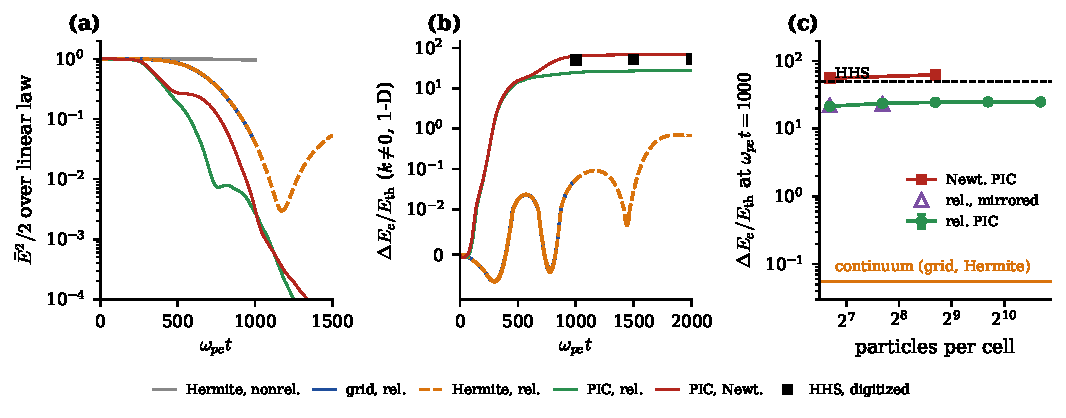
\includegraphics[width=\textwidth]{figures/fig_hhs.pdf}
\caption{Resonant drive $\vq=0.03$ (figure of the paper). (a) Mean-field energy over the exact linear law (trailing $200\,\wpe^{-1}$ mean) for the nonrelativistic Hermite model, the relativistic grid, the relativistic Hermite model and the relativistic and Newtonian PIC. (b) HHS measure of the $k\ne0$ electron energy change over $\Eth$ (symmetric logarithmic scale); squares: HHS Fig.~2 re-digitized. The continuum curves coincide to $\wpe t=1000$ and remain below $\sim1\,\Eth$ to $2000$. (c) Heating at $\wpe t=1000$ against particles per cell, with the relativistic plateau, the Newtonian PIC, mirrored loading, the HHS value and the continuum value.}\label{fig:c10-hhs}
\end{figure}
